The core of the tracking engine is a technique known as the
\emph{particle filter}.  The particle filter is a kind of Bayesian
filtering where one uses discrete hypotheses, also known as
\emph{particles}, to approximate continuous probability density
functions (PDFs) \cite{ProbRob}.  It builds upon the theory of
\emph{Markov processes} and the \emph{hidden Markov model}.

\section{Markov processes} A Markov process is a special case of a
stochastic process. For a Markov process, the next state depends only
on the present state and not on past states.  For this reason, a
Markov process is often said to be ``forgetful''.

In mathematical terms, a Markov process satisfies the following:
\begin{equation} p\left(Z_t|Z_{t-1} \wedge Z_{t-2} \wedge \dots \wedge
Z_0\right) = p\left(Z_t|Z_{t-1}\right),
\end{equation} $p\left(Z_t|Z_{t-1} \wedge Z_{t-2} \wedge \dots \wedge
Z_0\right)$ is the probability that the system will have state $Z_t$
at time $t$, given that the previous states where $Z_{t-1},
Z_{t-2},\dots, Z_0$. Figure \ref{fig:mp-graph} shows how the state $Z$
changes between time steps, depending on the previous state.

\begin{figure}
  \centering
  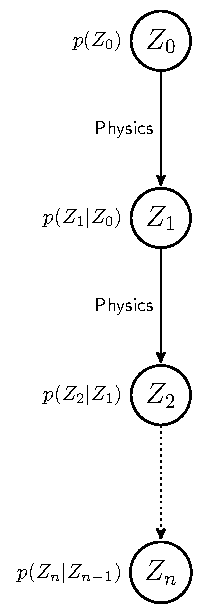
\includegraphics[width=0.175\textwidth]{mp-graph.pdf}
  \caption{Schematic image of a Markov process.}
  \label{fig:mp-graph}
\end{figure}

\section{The Hidden Markov Model}

The working principle of the particle filter is based on the
\emph{hidden Markov model} (HMM).  A HMM describes a Markov process
where we cannot measure the state directly - it is
``hidden''\cite{EncyclopediaMachineLearning}.  Instead we obtain an
\emph{observation} $I$\footnote{In this thesis, the observation is
always a grayscale \emph{image}, therefore the observation is denoted
$I$.}  of the state. This \emph{perception} is generally
non-deterministic, so we need to denote it as $p(I_t|Z_t)$ which is
the probability that we will observe $I_t$ if the state is
$Z_t$. Figure \ref{fig:hmm-graph} shows how the observation $I_t$ is
nondeterministic, but depends on the state $Z_t$.

\begin{figure}
  \centering
  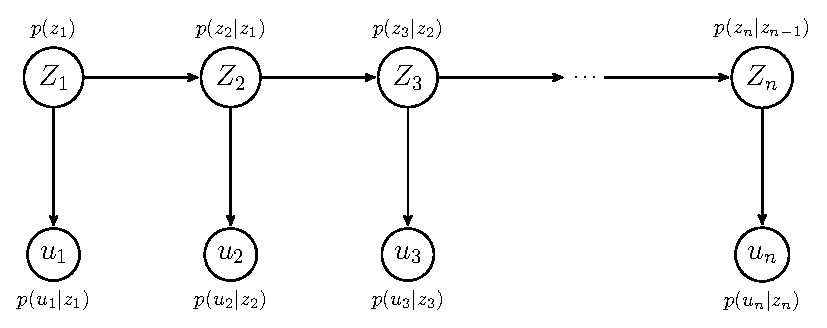
\includegraphics[width=0.35\textwidth]{hmm-graph.pdf}
  \caption{Schematic image of a hidden Markov model.}
  \label{fig:hmm-graph}
\end{figure}


\section{The Curse of Dimensionality} A phenomenon that becomes
apparent in high-dimensional spaces is the so-called ``Curse of
dimensionality'' \cite{EncyclopediaMachineLearning}.  The problem is
that the search volume grows exponentially with the number of
dimensions.  It originates from the fact that we need $\Ordo{C^n}$
samples to obtain a sample density of $C$ in a $n$-dimensional space.

The first consequence of this is that in order to approximate a
high-dimensional function one needs orders of magnitude more samples.

The other drawback with high dimensional space is the large
``borders'' of the sample-set compared to lower dimensional space
which results in orders of magnitude higher chance for an point one
want to approximate to fall outside the sample-set and needs to be
extrapolated instead of the better alternative of interpolation.

\begin{example} Figure \ref{fig:curse-of-dimensionality} shows 128
randomly scattered points in 1, 2 and 3 dimensions. Notice how the
density decreases with increasing dimension.
  \begin{figure}
    \begin{tabular}{rcl}
      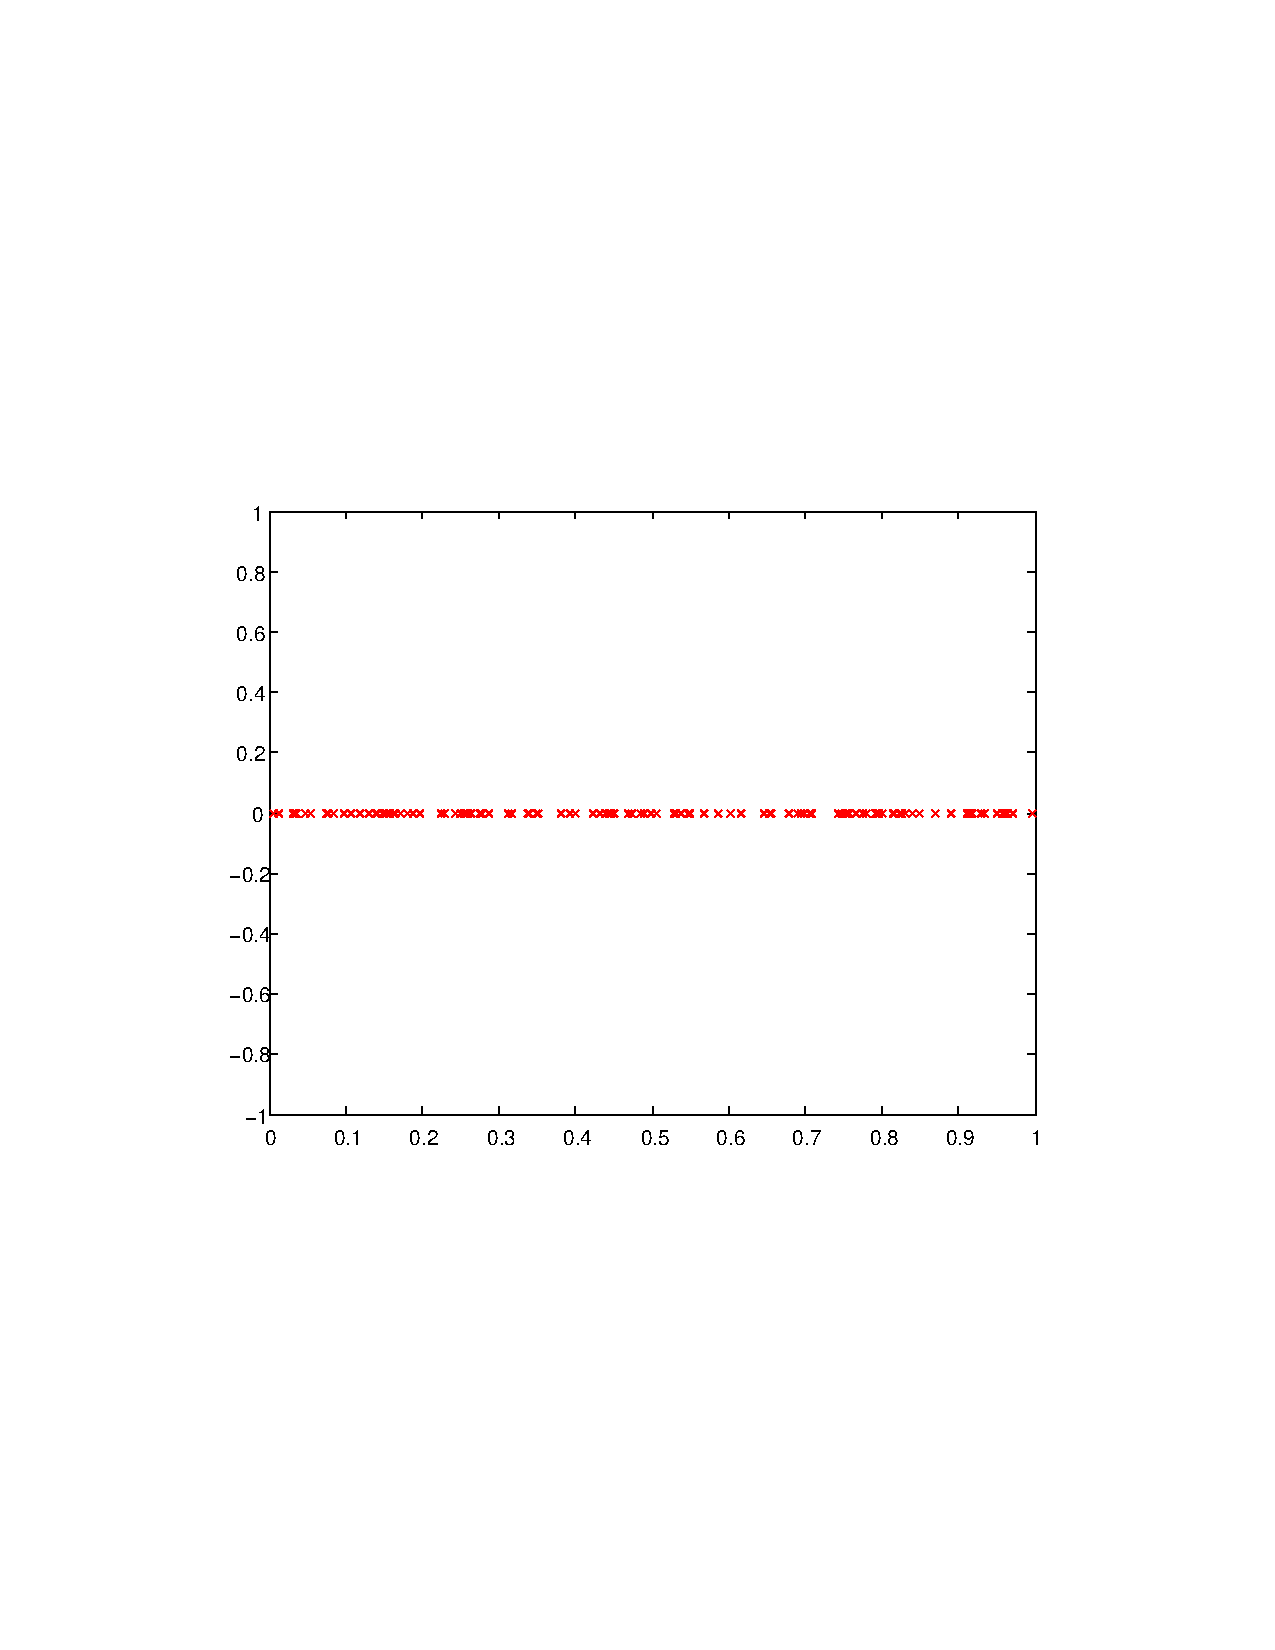
\includegraphics[scale=0.3,trim=4cm 4cm 4cm 4cm]{1D.pdf}&
      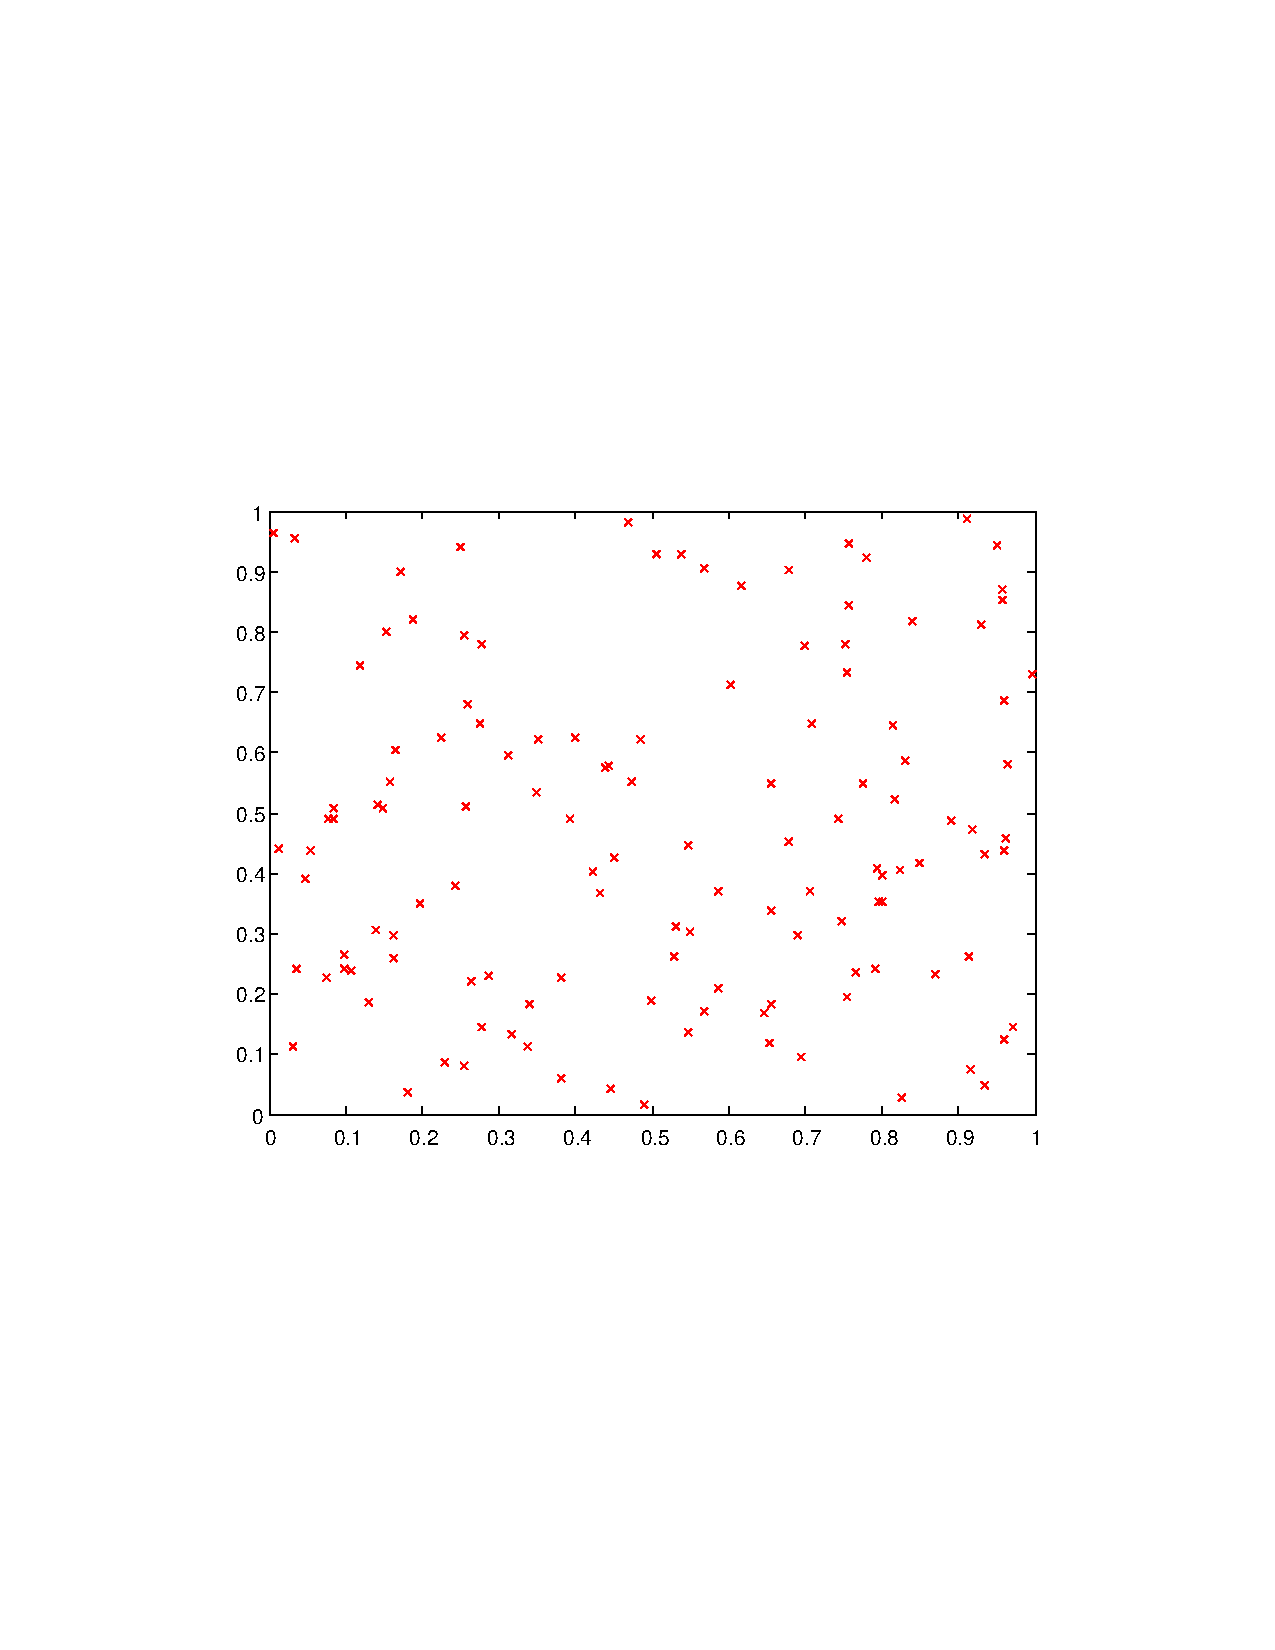
\includegraphics[scale=0.3,trim=4cm 4cm 4cm 4cm]{2D.pdf}&
      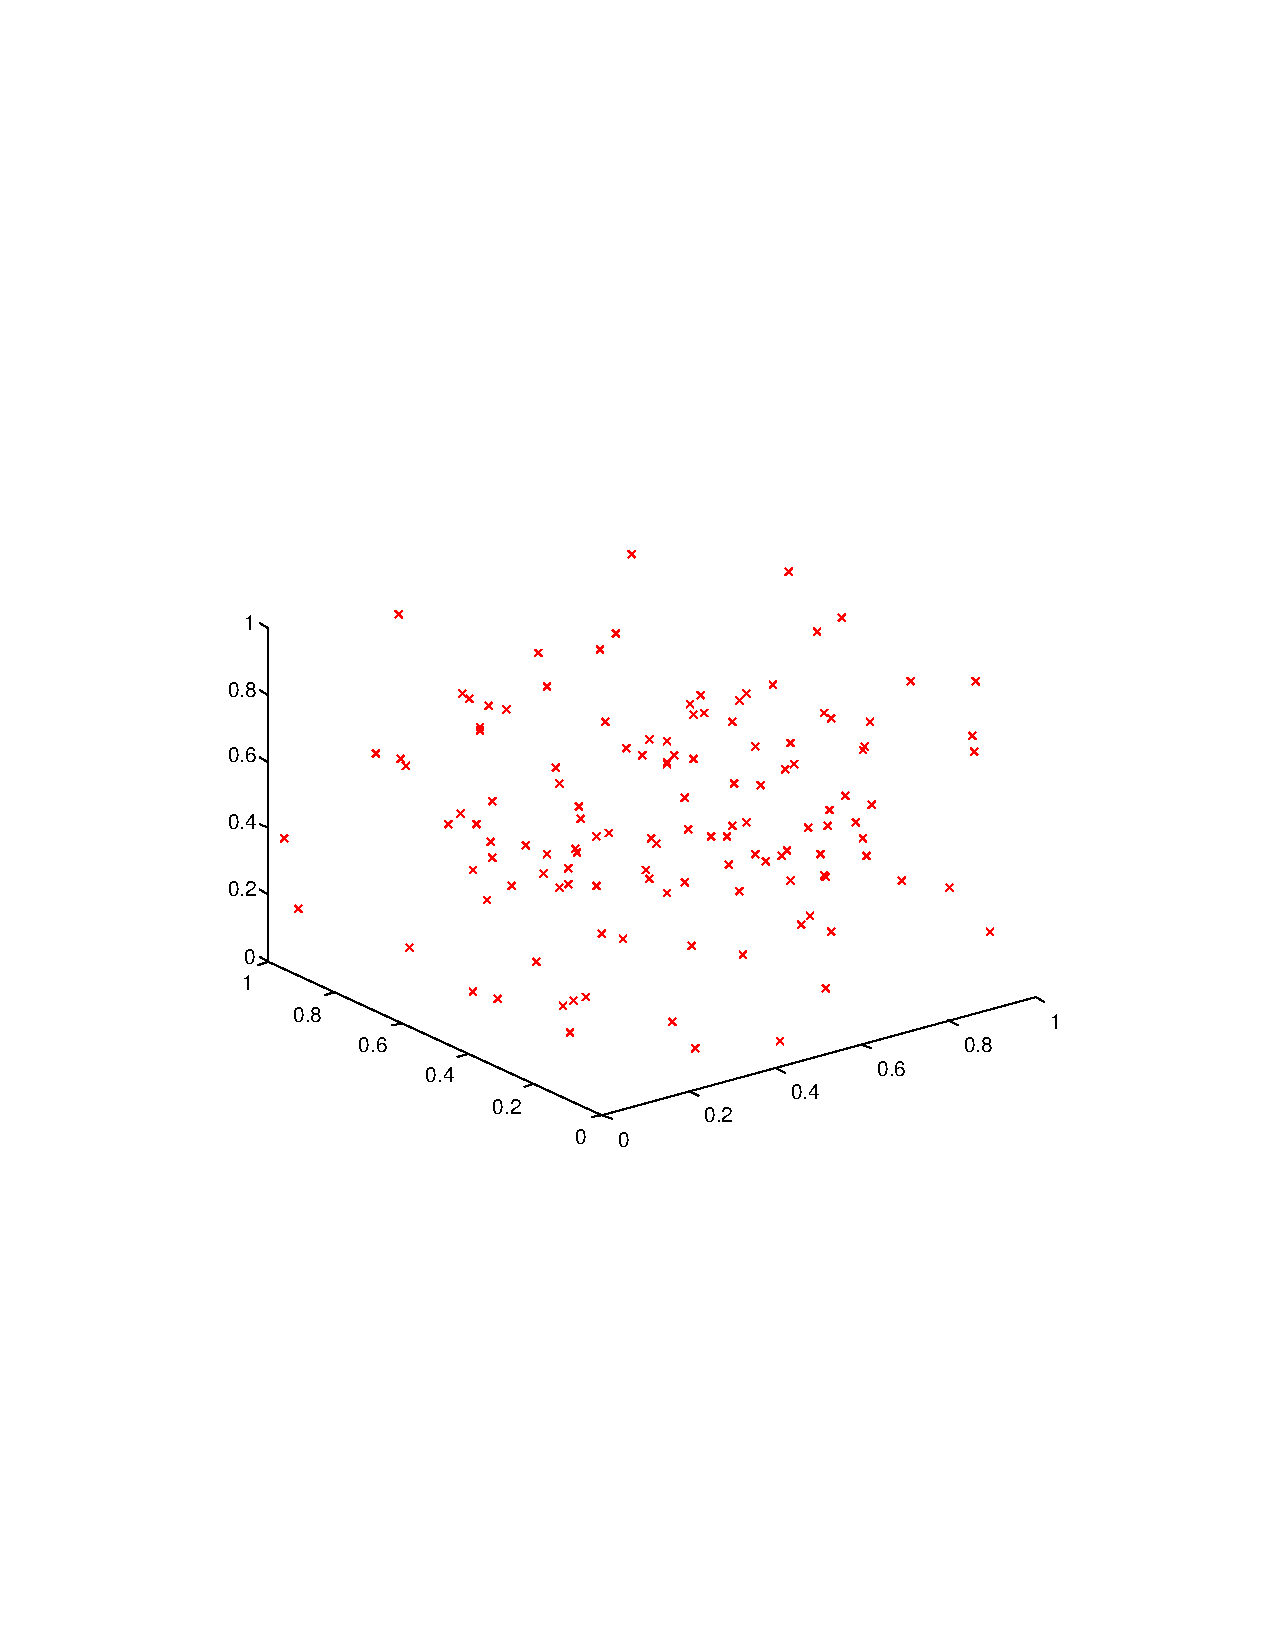
\includegraphics[scale=0.3,trim=4cm 4cm 4cm 4cm]{3D.pdf}
    \end{tabular}
    \caption{Plots of $128$ scattered samples in $1$, $2$ and $3$
dimensions, respectively.}
    \label{fig:curse-of-dimensionality}
  \end{figure}
\end{example}

\begin{example} For a $16$ DOF model one needs $10^{16}=10$
quadrillion datapoints to acquire a density of $10$ samples per unit
volume. Millions of gigabytes would be needed just to store the
samples.
\end{example}

\begin{example} In 2 dimensions it is sometimes feasible to use an
exhaustive search.  An example of this is the Hough transform
\cite{DigitalImageProcessing}, where the search is done through the
$\rho\theta$ space of line responses on images.
\end{example}

\subsection{Overcoming the Curse}
One way to overcome the curse in the context of tracking is to perform
a directed search, which could be done in one of the following ways:

\begin{enumerate}
\item Let the search be in an $n$ dimensional space with a grid of $g$
  grid lines in each direction. Use the information about the most
  recent\footnote{In the Bayesian case, the most recent estimate}
  location and assume that the tracked object cannot travel more than
  $R < g$ grid steps in one time step.  This reduces the volume of the
  (discrete) search space from $\Ordo{g^n}$ to $\Ordo{R^n}$.
\item With prior knowledge of how the tracked objects
  move\footnote{Such as the state transition probabilites
    $\cprobnext{Z}$ in a HMM} we can direct our search to specific
  regions in the state space, depending on how probable it is for the
  tracked object to be located there. This reduces the size of the
  search space depending on how sure we are of the previous state.
\end{enumerate}

For a system whose dynamics is unknown, it may be difficult to achieve
the first of these two. The \emph{particle filter} is a general
technique that employs the second one, by first \emph{predicting} the
next state and then \emph{filtering} the predictions depending on how
probable they are.


\section{The Particle Filter}

The \emph{particle filter} is a technique for reducing the size of the
search space. It uses a finite set $X_t$ of hypotheses to approximate
the PDF $\cprobnext{Z}$ of a HMM. The hypotheses $X_t$ are also
refered to as \emph{particles}, thereby the term ``particle filter''.

\begin{figure}
  \centering
  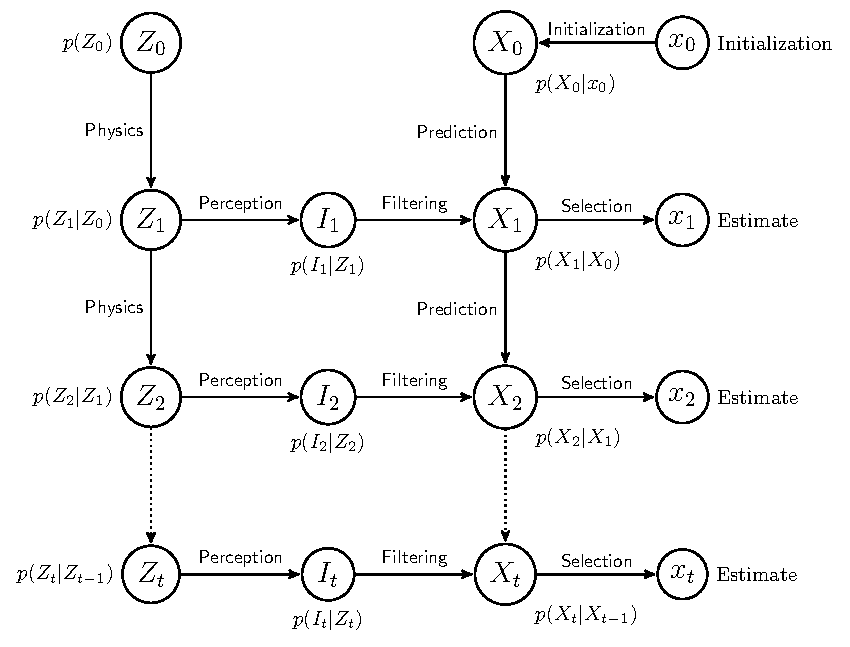
\includegraphics[width=0.8\textwidth]{hmm-pf-graph.pdf}
  \caption{Schematic image of the particle filter alongside a HMM.}
  \label{fig:hmm-graph}
\end{figure}

Figure \ref{fig:hmm-graph} shows the principle of the particle filter
working alongside a hidden Markov model. The following is the core
function of the particle filter:

\begin{quote}
  \emph{The particle filter attempts to approximate the PDF
    $\cprobnext{Z}$ as a set $X_t$ of discrete hypotheses.}
\end{quote}

More particles mean greater accuracy, since the PDF can then be
approximated more closely. However, using many particles increses
computational cost.  Therefore the number of particles is an important
trade-off.  The particle filter employs a few tricks to \emph{filter}
the hypotheses, tending to keep probable ones and throwing improbable
ones away, in order to intelligently reduce the number of particles
needed for a good approximation. The filter works in four steps:

\begin{description}
\item[Prediction] The hypotheses $X_{t-1}$ are updated in the
  \emph{prediction} step to an approximation $\bar{X}_t$ of
  $\cprobnext{Z}$.  This is done by drawing new samples
  $\cprobnext{x}$, for each $x_{t-1}$ in $X_{t-1}$.
\item[Perception] By measuring the state of the system, we gain an
  \emph{observation} $I_t \sim \cprob{I_t}{Z_t}$ of the state $Z_t$.
\item[Filtering] The observation $I_t$ of the system is then used for
  filtering bad hypotheses out of $\bar{X}_t$.  We draw samples $X_t$
  from $\bar{X}_t$ with probabilities given by
  $\cprob{I_t}{\bar{X}_t}$. The result will be a surjection, where
  $X_t$ will be a subset of $\bar{X}_t$ where more probable hypotheses
  appear multiple times.<ref:problem without sigma> For this reason,
  this is also known as the \emph{resampling} step. The set $X_t$ is
  the \emph{belief}, our approximation of $\cprobnext{Z}$.
\item[Selection] Finally, we produce a single hypothesis $x_t$ from
  $X_t$ as our \emph{estimate} of the state $Z_t$. Assuming $X_t$ is a
  good approximation of $\cprobnext{Z}$, and that $\cprobnext{Z}$ is
  unimodal, the means value of $X_t$ is a good estimate since it
  approximates the expectation of $\cprobnext{Z}$.  If $\cprobnext{Z}$
  is multimodal, however, the mean could be a bad estimate since the
  expectation may be very improbable.
\end{description}

The reason why this works is the following theorem, which is Theorem
3.1 in \cite{Hedvig} with some modifications to notation:

\begin{theorem}
  Given the PDFs $\cprobnext{x}$, $\cprob{I_t}{x_t}$ and
  $\cprob{x_{t-1}}{I_{t-1} \wedge \dots \wedge I_0}$, the PDF
  $\cprob{x_t}{I_t \wedge \dots \wedge I_0}$ can be expressed as

\begin{equation}
  \cprob{x_t}{I_t \wedge \dots \wedge I_0} = \kappa \cprob{I_t}{x_t} \int{ \cprobnext{x}\cprob{x_{t-1}}{I_{t-1} \wedge \dots \wedge I_0} \mathrm{d}x_{t-1}},
  \label{thm:pf-grand}
\end{equation}
where $\kappa$ is a normalization constant

For the proof of this, see \cite{Hedvig}.

\end{theorem}

Let's sketch out the connection between this and what we've done so
far. <<THIS WILL BE EDITED.>> For a more rigorous derivation, see chapter 4 of \cite{ProbRob}.

In this thesis, $\cprob{x_t}{I_t \wedge \dots \wedge I_0}$ is
approximated as the set $X_t$ of hypotheses. Substituting this into
\eqref{thm:pf-grand} and replacing the integral with a sum yields

\begin{equation}
  X_t = \kappa \cprob{I_t}{x_t} \sum { \cprobnext{x} X_{t-1} }.
\end{equation}

Note that this is horrible abuse of notation, but from here we can
take the step to

\begin{equation}
  X_t \sim \cprob{I_t}{x_t} \cprobnext{x}
\end{equation}

\subsection{The Particle Filter algorithm}
\begin{table}
  \begin{codebox}
    \Procname{$\proc{Particle-Filter} (X_{t-1},I_t)$}
    \li $\bar{X}_t \gets \emptyset$
    \li \ForEach $x_{t-1} \in X_{t-1}$
    \li \Do
    \li $x_t \gets \proc{Predict}(x_{t-1})$
    \li $w \gets \proc{Importance}(x_t,I_t)$
    \li Append $\left<x_t, w\right>$ to $\bar{X}_t$
    \End
    \li
    
    \li $X_t \gets \emptyset$
    
    \li \While $\abs{X_t} < \abs{\bar{X}_t}$
    \li \Do
    \li Take $\left<x_t, w\right>$ from $\bar{X}_t$ with probability $\propto w$
    \li Append $x_t$ to $X_t$
    \End
    \li \Return $X_t$
  \end{codebox}
  \caption{The particle filter algorithm.}
  \label{alg:pf}
\end{table}

Table \ref{alg:pf} shows the particle filter algorithm. Note that the
functions \textsc{Predict} and \textsc{Importance} are unspecified -
they are problem specific. They correspond to the PDF $\cprobnext{x}$
and $\cprob{I_t}{x_t}$, respectively.

% We draw a set $\bar{X}_t = \xtmN{x}{t}{i}{N}$ of samples from
% $p$. These samples roughly represent a PDF for the current state
% $x_t$, but we have yet to consider our observation.  Therefore, we
% will create a new PDF weighted by how probable the observation $z_t$
% is. For each $x_t^m$, we let $w_t^m := q\left(z_t |
%   x_t\right)$. This defines a discrete PDF where $x_t^m$ is assumed
% with a probability proportional to $w_t^m$. From this final
% distribution we again draw $N$ samples $X_t$, which will be our
% estimate of the current state.  The elements $x_t^m$ are referred to
% as \emph{particles} and the set $X_t$ as the \emph{belief at time
%   $t$}.

In this thesis, the real $x_{t-1}$ is not known. Rather $x_{t-1}$ is
estimated with a set $X_{t-1}$ of $N$ particles.

\section{Visual Cues}
\begin{quote}
    The biggest problem with computer vision is that computers do not have
    vision, only a data input device in the form of a camera.
\end{quote}
A \emph{visual cue} is an image transformation $\phi$ that extracts
some property of the image, such as intensity
\footnote{In our case this is possible since we have an homogenous object
in the form of a backlit rodent}, edges, ridges\cite{Hedvig} or different 
refinements as in section \ref{prep-real}.

\section{Response}

\begin{definition}
    A \emph{response} is how much a hypothesis matches an image. The similarity measure for hypothesis response this thesis is defined by
    \begin{equation}
        \label{eq:response}
        \Response{x_t}{I_t}{\phi} = \sum{\phi(R(x_t))*\phi(I_t)} \in \RR^+
    \end{equation}
    where $\Response{x_t}{I_t}{\phi}$ will denote the response. 
    \footnote{The denotation $\Response{\cdot}{\cdot}{\phi}$ for response was choosen to show the similaritise with inner product.}

\end{definition}

Assuming $R$ renders $x_t$ perfectly and that $I_t$ does not have clutter, the maximum response will uniquely
\footnote{Disregarding the phenomena of having $\exists x_a\neq x_b : R(x_a)=R(x_b)$},
be when the two underlying models coinside by theorem \ref{thm:response_max}.
How nice the response peak is is highly dependent on all the terms in \eqref{eq:response}.

\begin{theorem} %TODO svagare?
  \label{thm:response_max}
  Let $f$ be a positive Riemann function with finite support,
  defined on a set $\Omega$. Then
  \begin{equation}
    \argmax{\bar{e}}
    \left( \int\limits_{\Omega}{f(\bar{x})f(\bar{x}-\bar{e})} \right)
    =0
    \label{thm:response-max-eqn}
  \end{equation}
\end{theorem}
\begin{proof}
  Firstly define the window function as

  \begin{IEEEeqnarray*}{s"r?c?l}
    & W_a^b(x) & = &
    \begin{cases}
      0,~& x<a\\
      1,~& a \leq x \leq b\\
      0,~& x>b
    \end{cases}\\

    Multiplication: &
    (W_a^bW_c^d)(x) & = & W_{\max(a,c)}^{\min(b,d)}(x)\\

    Translation: &
    W_a^b(x-e) & = & W_{a+e}^{b+e}(x)\\

    Integration: &
    \int\limits_{\RR}{W_a^b(x)dx} & = & \Theta(b-a).
  \end{IEEEeqnarray*}
  
  \begin{IEEEeqnarray*}{L?c?l}
    \argmax{e}\left( \int{W_a^b(x)W_a^b(x-e)} \right) &=& \\
    \argmax{e}\left( \int{W_a^b(x)W_{a+e}^{b+e}(x)} \right) &=&\\
    \argmax{e}\left( \int{W_{\max(a,a+e)}^{\min(b,b+e)}(x)} \right) &=&\\
    \argmax{e}\left( \Theta(\min(b,b+e)-\max(a,a+e)) \right) & = & 0.
  \end{IEEEeqnarray*}
  
  This trivially holds for superposition of windows, since all windows
  will scale and translate the same way.  With a finite support, $e=0$
  is the only solution. Additionaly, this also holds in higher finite
  dimensions since we can just repeat the process one dimension at a
  time.
    
  All riemann functions with compact support can be written as a superposition of finite number of finite windows
  like this
  \begin{equation*}
    f(x)=\sum{c_iW_{a_i}^{b_i}(x)},
  \end{equation*}
  and therefore \eqref{thm:response-max-eqn} holds for any Riemann function $f$.
  
\end{proof}

Assuming that a whisker has one fix point of origin<ref:analysis(this is not
the case really)> we have the boundary condition $whisker(0)=0$

"There are many metrics by which a model may be assessed." - Encyclopedia
(>model evaluation)

"
==Model selection
Model selection is the process of choosing an appropriate mathematical model
from a class of models.
" - Encyclopedia 
The class being all functions with f(0)=0,contioiuns(or stronger?) and finite number of parameters



